\chapter{Humanoids and steerable WMRs}
\label{ch:humanoids-and-swmrs}
The idea of building a machine that replicates the human body, and is capable 
of executing the same tasks that we do, has fascinated humanity since forever.
The earliest ideas can be dated back to the third century BC, when the 
Chinese philosopher Lie Yokou described a humanoid automaton constructed of 
leather and wood, capable of moving all parts of its body
\cite{Needham1956ScienceandCivilisationinChinaVol2}. In the first century AD,
the greek mathematician and engineer Heron of Alexandria described a machine 
capable of pouring wine for party guests \cite{Alexandria2015Pneumatica}.
In 1206, the Muslim engineer Ismail al-Jazari published a book describing 
about one hundred mechanical devices, including automata performing different 
facial expressions \cite{AlJarari1206BookofKnowledge}. Among these ancient
automata, the most famous one is undoubtedly Leonardo's mechanical knight 
(or Leonardo's robot), a humanoid automaton in a suit of a knight's armor
build by Leonardo Da Vinci in 1495 \cite{Moran2006TheDaVinciRobot}.
Even though the history of robots started many centuries ago, the word ``robot''
first appears only in 1920 in the science-fiction play R.U.R.
(Rossum's Universal Robots) \cite{Capek1920RUR}, written by the Czech writer
Karel {\v C}apek.
In the last century, robots have become part of our world. Apart the adoption 
of robots in the industry, and the use of robots in academia, we are now 
used to see robots in movies (e.g., C-3PO in Star Wars,
Fig. \ref{fig:introduction:robots-in-history}), in animation (e.g., The Iron
Giant, Bender and Baymax, Fig.
\ref{fig:introduction:robots-in-animation}), and in books (Isaac Asimov
introduced the Three Laws of Robotics in his 1942 ``Runaround'' story).

This chapter gives a brief overview on the main developments in the field of 
robotics happened in the last 50 years, focusing in particular on humanoids
(from the WABOT-1 to the commercialization of humanoids)
and steerable WMRs (from interaction with humans to space exploration),
which are the type of platforms used in the following chapters.

\begin{figure}
    \centering
    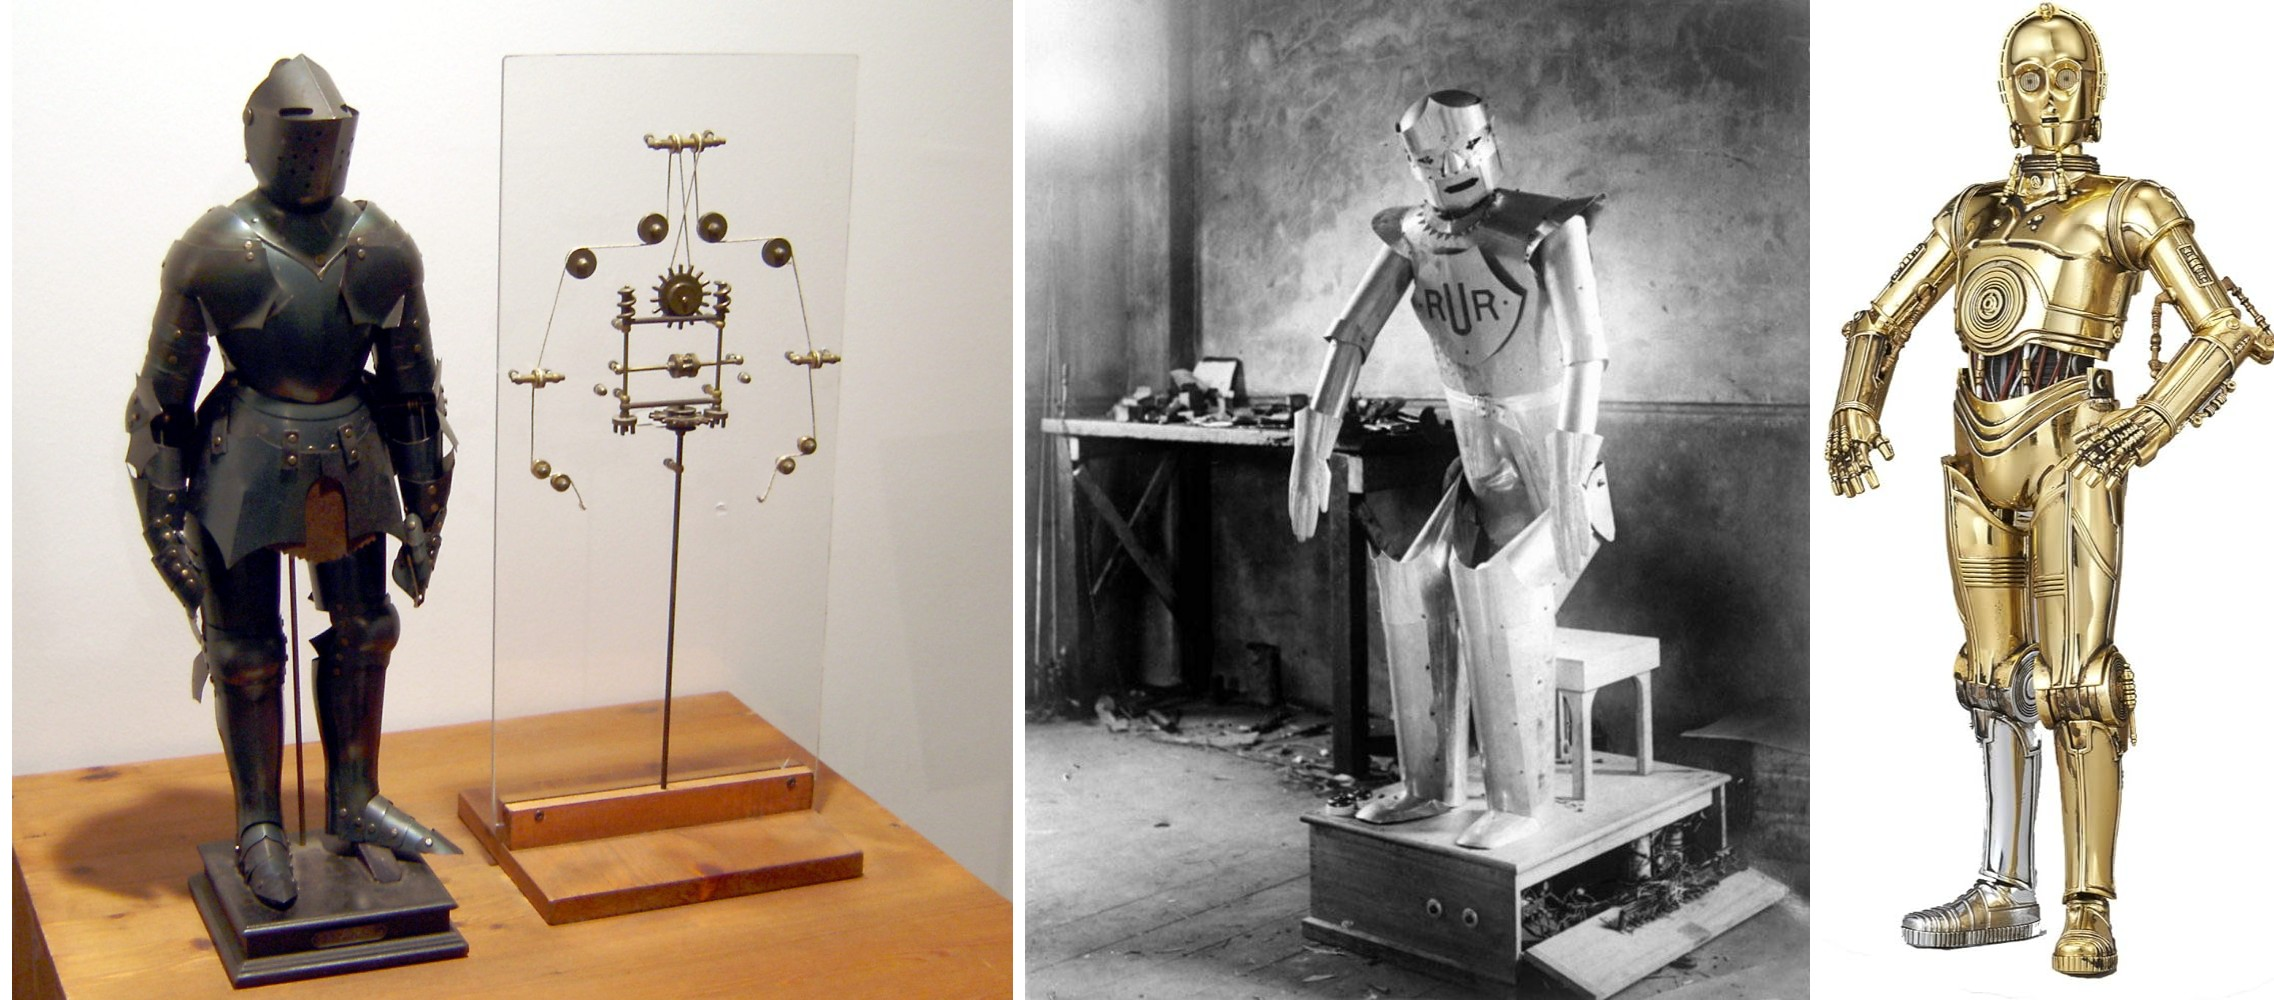
\includegraphics[width=\textwidth]{figures/01-introduction/robot-history.jpg}
    \caption{From left to right: Leonardo's robot, constructed by Leonardo Da
        Vinci in 1495 \cite{Moran2006TheDaVinciRobot};
        R.U.R. (Rossum's Universal Robots) by Karel {\v C}apek introduced 
        the word ``robot'' in 1920 \cite{Capek1920RUR};
        C-3PO, the famous humanoid robot from the Star Wars Cinematic Universe
        \cite{StarWars1977}.
    }
    \label{fig:introduction:robots-in-history}
\end{figure}

\begin{figure}
    \centering
    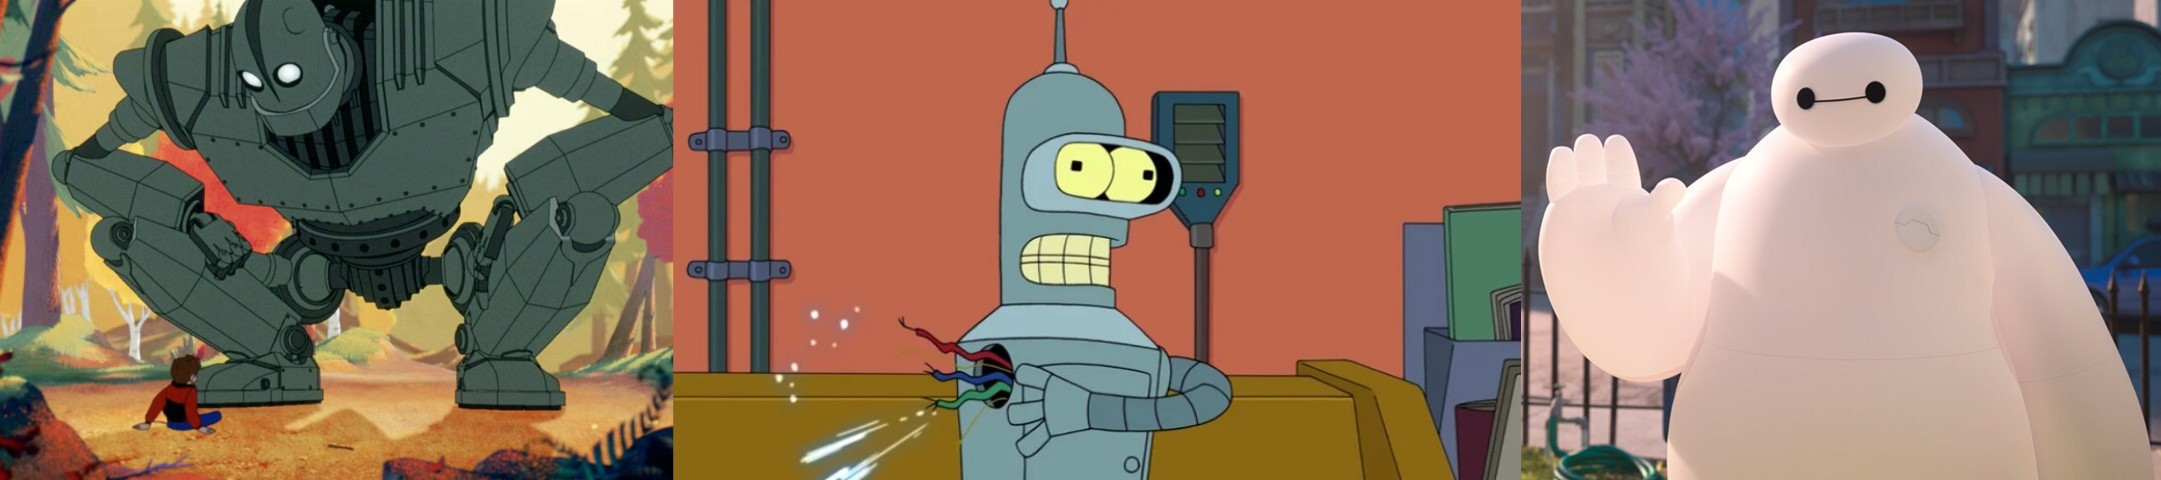
\includegraphics[width=\textwidth]{figures/01-introduction/robots-in-animation.jpg}
    \caption{Humanoid robots in animation. From left to right:
        The Iron Giant (1999) \cite{TheIronGiant1999},
        Bender from Futurama (1999) \cite{Futurama1999}, and
        Baymax from Big Hero 6 (2014) \cite{BigHero62014}.
    }
    \label{fig:introduction:robots-in-animation}
\end{figure}

\subsubsection{First prototypes: WABOT-1 and WABOT-2}
The first anthropomorphic robot ever developed is the WABOT-1
\cite{Kato1973TheWABOT1}, whose project started in 1967 and completed in 1972.
The robot (Fig. \ref{fig:introduction:WABOTs}), was constituted by a limb-control
system, which allowed it to walk, and a conversation system, 
which allowed it to communicate with a person in Japanese. The development 
continued with the WABOT-2 \cite{Kato1987WABOT2}, introduced in 1984,
a musician robot able to play a keyboard instrument (Fig.
\ref{fig:introduction:WABOTs}) and read a musical score with his eyes. The WABOT
project is considered as a turning-point in the development of humanoids, as it 
introduced the first programmable multi-purpose humanoid robot.

\begin{figure}
    \centering
    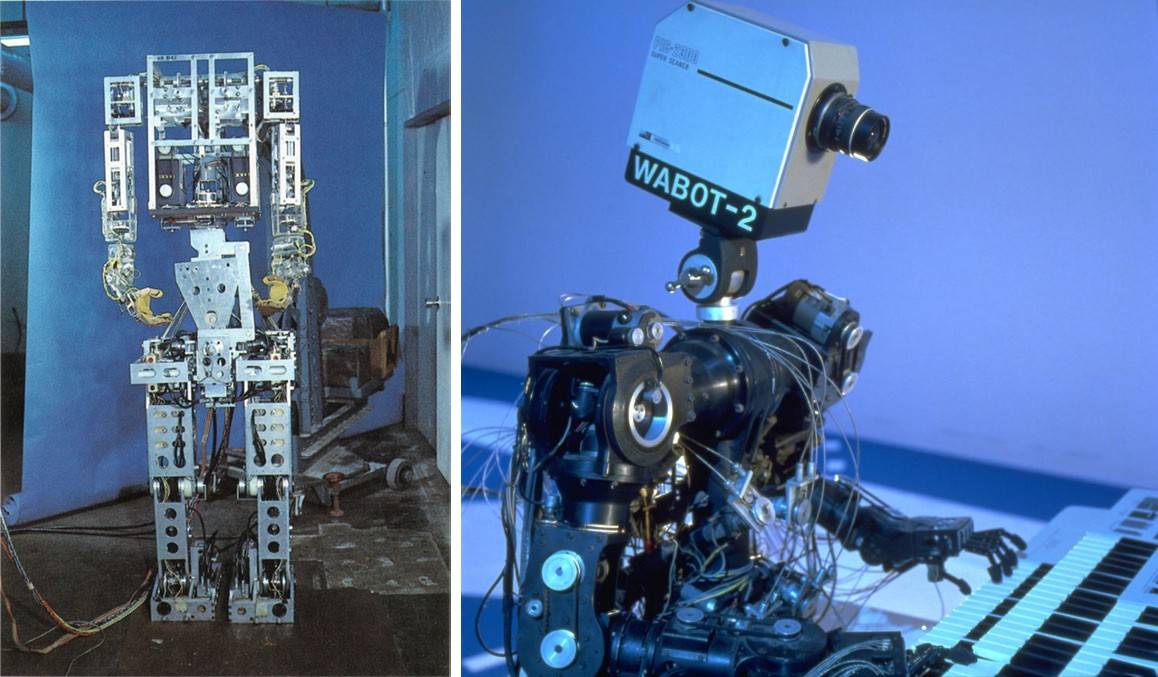
\includegraphics[width=0.7\textwidth]{figures/01-introduction/WABOTs.jpg}
    \caption{From left to right: the WABOT-1 (1972), which is the first anthropomorphic robot
        ever developed \cite{Kato1973TheWABOT1}, and the WABOT-2 (1984)
        playing a keyboard \cite{Kato1987WABOT2}.}
    \label{fig:introduction:WABOTs}
\end{figure}

\subsubsection{Honda humanoids: E series, P series and ASIMO}
During the 80s and the 90s, the development of humanoids was mainly dominated
by Honda, which introduced his first humanoid, E0, in 1986. E0 had 6 degrees
of freedom, and it could walk slowly (it needed around 5 seconds to complete 
a step) in a straight line. This model was further developed into the E-series 
robots (E1, introduced in 1987, to E6, introduced in 1993), which could walk 
faster, balance autonomously, avoid obstacles and climb stairs. The E6 was 
much heavier (150 kg) and taller (174 cm) with respect to the E0 (whose 
weight was 16.5 kg and height was 101 cm).
The development of Honda humanoids evolved into the P series. The first of these 
robots, the P1, had 30 degrees of freedom, it
was 191 cm tall and it weighed 175 kg. The P1 was kept secret until the 
announcement of the P2 in 1996, which is described in detail in
\cite{Hirai1998HondaP2}.

In 2000, Honda introduced ASIMO (Advanced Step in Innovative Mobility)
\cite{Sakagami2002ASIMO}, a humanoid robot capable of walking and running 
up to 9 km/h. Among its physical capabilities, ASIMO was able to handle trays 
and carts, and pour drinks. Moreover, because of its voice and image recognition
technologies, it was able to interact with people, giving presentations and 
providing explanations of exhibits \cite{Shigemi2019ASIMOandHumanoidRobotResearchatHonda}.
The development of ASIMO has ceased in 2018, and its last public appearence
took place in 2022.

\begin{figure}
    \centering
    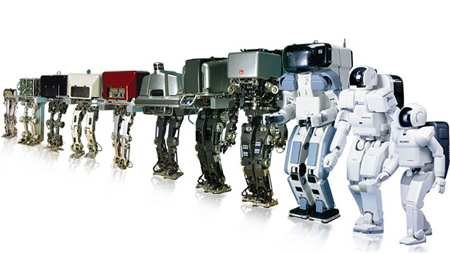
\includegraphics[width=0.7\textwidth]{figures/01-introduction/The-ASIMO-humanoid-robot-history.png}
    \caption{Honda E series (E0 in 1986 to E6 in 1993) robots, Honda P series (P1 in
        1993 to P3 in 1997) robots, and ASIMO (2000)
        \cite{Shigemi2019ASIMOandHumanoidRobotResearchatHonda}.}
    \label{fig:introduction:ASIMO-humanoid-history}
\end{figure}

\subsubsection{2000s: humanoids of the new millenium}
Apart from ASIMO, the 2000s have seen the introduction of many humanoids of 
different dimension and cost, which shaped the technology of today's humanoids.
In 1998, Japan's Ministry of Economy, Trade and Industry started the Humanoid
Robotics Project (HRP), together with Kawada Industries, the National
Institute of Advanced Industrial Science and Technology (AIST) and Kawasaki
Heavy Industries, Inc. The project started with the Honda P3, which evolved 
during the decade into the HRP-2 \cite{Kaneko2004HRP2}, the HRP-3
\cite{Kaneko2008HRP3}, the HRP-4 \cite{Kaneko2011HRP4} (shown in Fig.
\ref{fig:introduction:robots-in-2000}) and the HRP-4C
\cite{Kaneko2009HRP4C}. These robots have been used in all sort of applications,
such as ladder climbing in industrial facilities \cite{Vaillant2016AuRo}, and aircraft manufacturing
\cite{Kheddar2019AircraftManufacturing}.

In 2006, the private company PAL Robotics introduced REEM-A, a humanoid designed to 
play chess, that could also walk and speak. The REEM project continued with 
the REEM-B \cite{Tellez2008REEMB}, which was introduced in 2008. The year 2006 
has seen the introduction of two other humanoids which are still used nowadays:
the NAO from Aldebaran \cite{Gouaillier2008NAOHumanoid}, used from healthcare
scenarios \cite{Cifuentes2020SocialRI} to soccer competitions \cite{Kitano1997RoboCupTR},
and the iCub \cite{Metta2010iCubHumanoid}, used mainly for research in 
cognitive robotics.

\begin{figure}
    \centering
    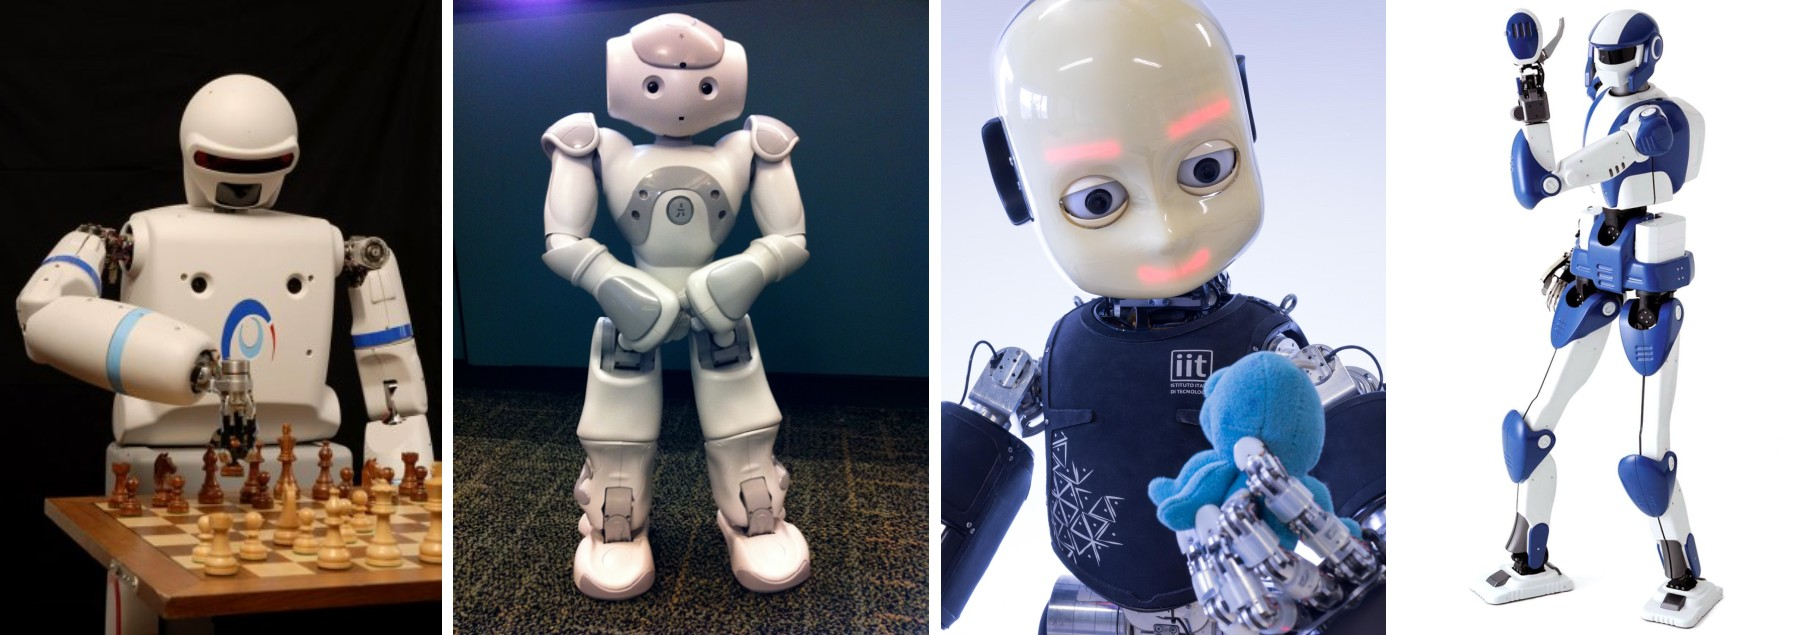
\includegraphics[width=\textwidth]{figures/01-introduction/robots-in-2000.jpg}
    \caption{Some of the humanoid robots developed in 2000s. From left to right:
        Aldebaran NAO \cite{Gouaillier2008NAOHumanoid},
        PAL Robotics REEM-B \cite{Tellez2008REEMB},
        iCub \cite{Metta2010iCubHumanoid}, and
        HRP-4 \cite{Kaneko2011HRP4}.
    }
    \label{fig:introduction:robots-in-2000}
\end{figure}

\subsubsection{2010s: DARPA robotics challenge}
The development of humanoid robots in 2010s was mainly shaped by the DARPA
Robotics Challenge \cite{Atkeson2018DARPARoboticsChallenge}, a competition 
organized by the US Defence Advanced Research Projects Agency in 2012, which 
had the objective to develop semi-autonomous humanoid robots to be deployed
in disaster scenarios. The competition consisted in solving several tasks,
such as driving a vehicle, opening a door, climbing an industrial ladder, 
using a tool to break through a concrete panel, and turn on a valve.
Amidst the robots used during the challenge, we can find the ATLAS by 
Boston Dynamics (Fig. \ref{fig:introduction:robots-in-2010}), the WALK-MAN 
developed by Italian Institute of Technology \cite{Tsagarakis2017WALKMAN},
and DRC-HUBO+ \cite{Jung2018DRCHUBO} from team KAIST, who won the challenge 
by completing all the tasks in the shortest time.

Among the other humanoid robots developed in this decade, DLR designed TORO
\cite{Englsberger2014TORO} for the study of walking and multi-contact 
balancing, NASA designed Valkyrie \cite{Radford2015Valkyrie} for advancing 
human spaceflight and extraterrestrial exploration, and PAL Robotics designed 
TALOS (Fig. \ref{fig:introduction:robots-in-2010}), a research platform mainly
targeted for industrial applications \cite{Stasse2017TALOS}.

\begin{figure}
    \centering
    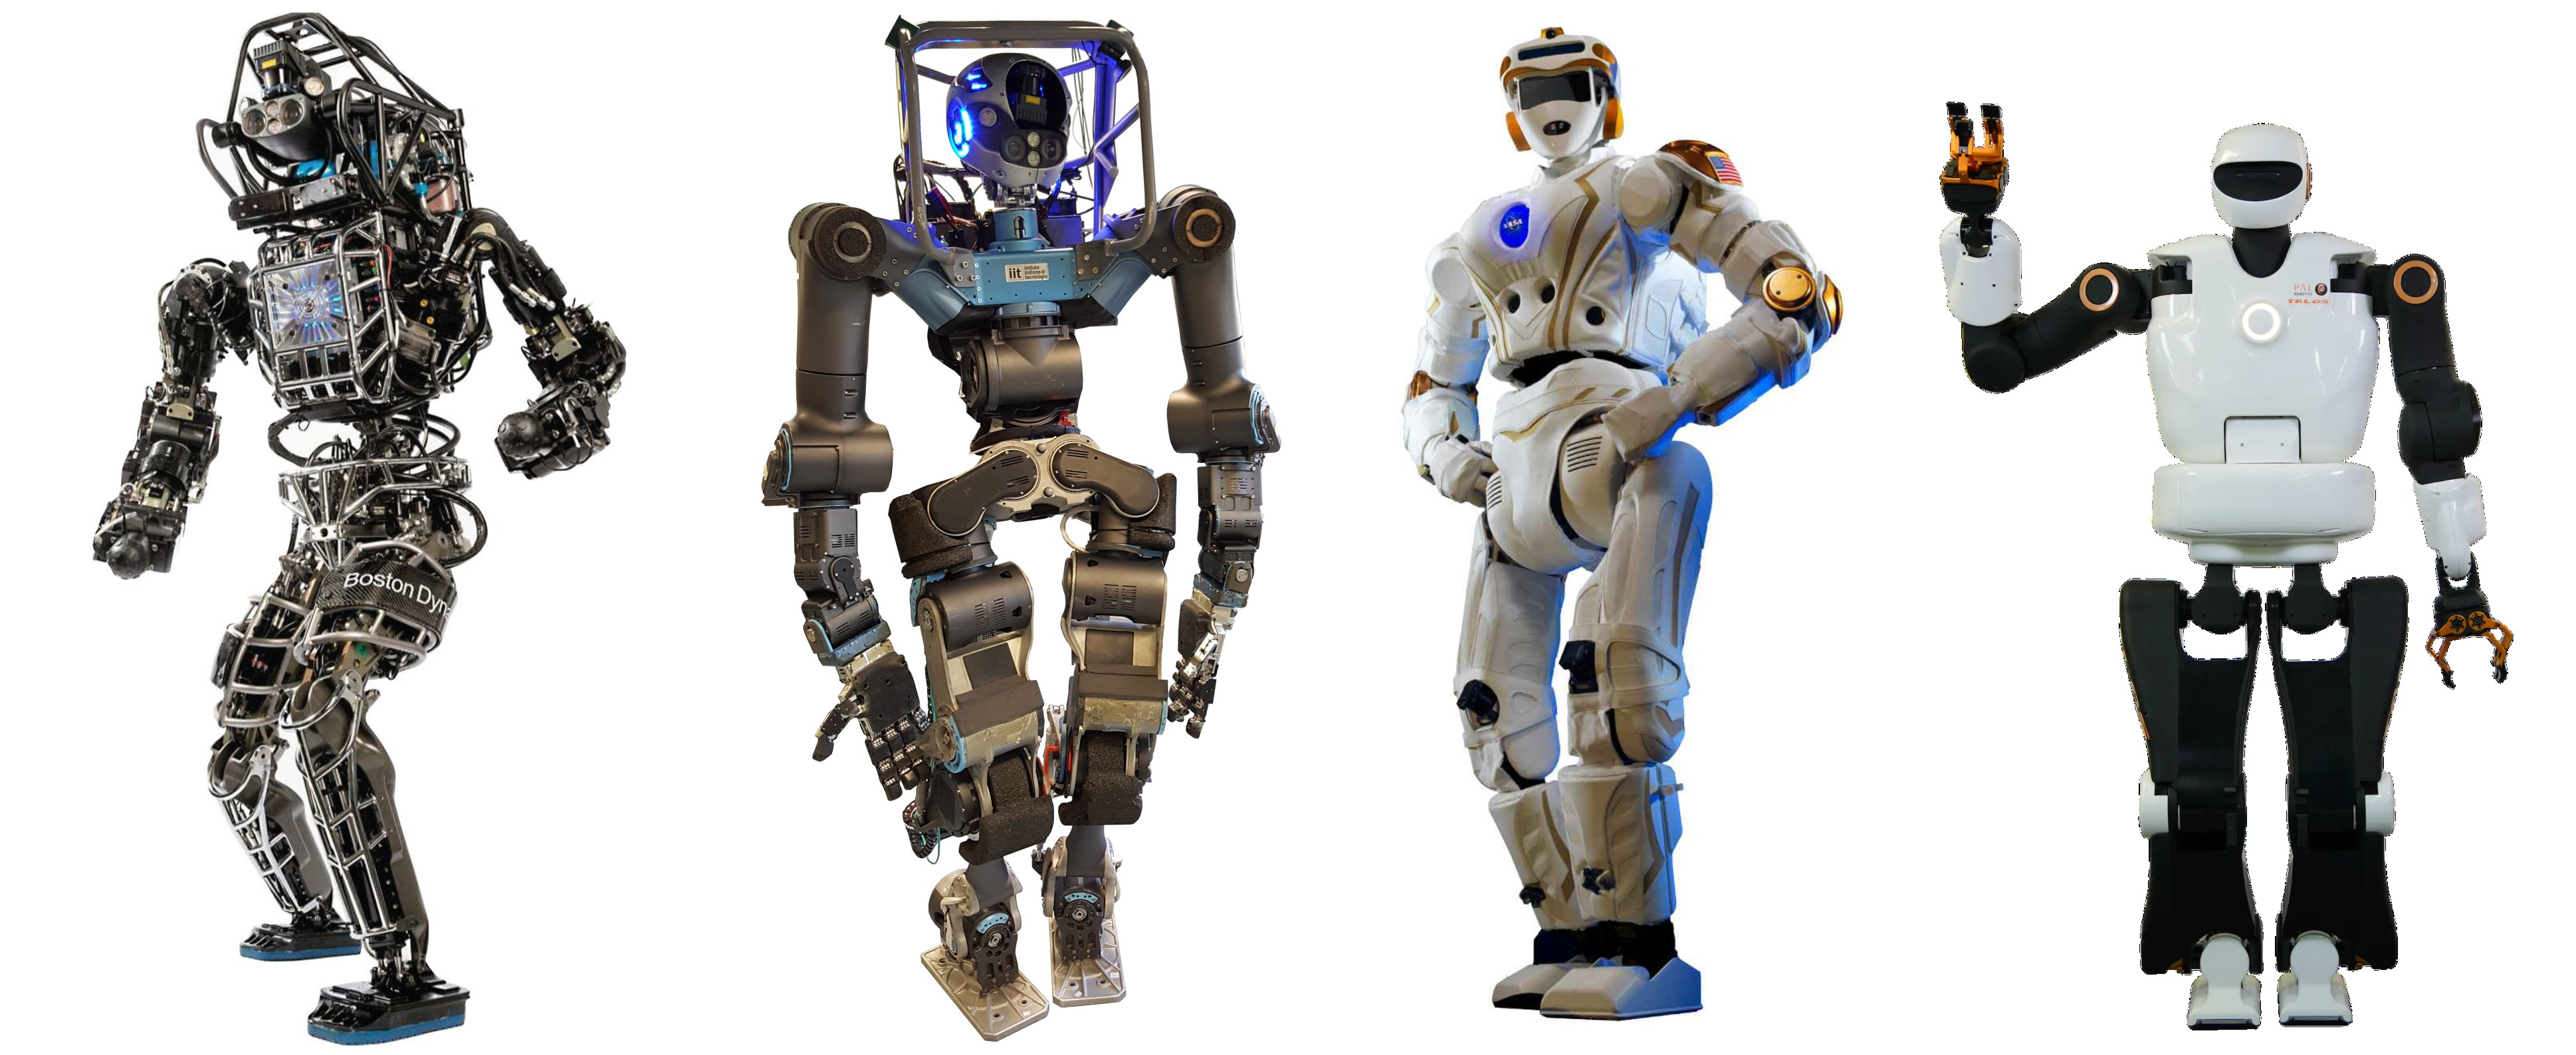
\includegraphics[width=\textwidth]{figures/01-introduction/robots-in-2010.jpg}
    \caption{Some of the humanoid robots developed in 2010s. From left to right:
        Boston Dynamics ATLAS,
        WALK-MAN \cite{Tsagarakis2017WALKMAN},
        NASA Valkyrie \cite{Radford2015Valkyrie}, and
        PAL Robotics TALOS \cite{Stasse2017TALOS}.}
    \label{fig:introduction:robots-in-2010}
\end{figure}

\subsubsection{2020s: humanoid robots as commercial products}
The technology of humanoids is mature enough, and this is reflect by the 
increasing number of companies interested in building humanoid robots, and the 
large investments in robotics companies\footnote{Just to give an example,
in February 2024, Figure AI has raised \$675 million in funding, reaching 
a valuation of \$2 billion.}.

Among the humanoids currently developed by private companies, we have Digit 
by Agility Robotics (Fig. \ref{fig:introduction:robots-in-2020}), Optimus by
Tesla, Apollo by Apptronik, Figure 01 by Figure AI, NEO by 1X, Phoenix by 
Sanctuary AI, H1 by Unitree, and GR-1 by Fourier Intelligence. All these 
humanoids are being developed with one common idea in mind: they must be 
general-purpose. Indeed, the tasks they are expected to perform vary from 
moving packages in a factory, unloading trailers, palletization,
last mile delivery to automotive production, and home assistance.

In the near future, we can thus expect to see an even more rapid growth in 
humanoid robot technologies, and the introduction of humanoids in a vast 
number of industries, revolutionizing the way we work, interact,
and experience the world around us.

\begin{figure}
    \centering
    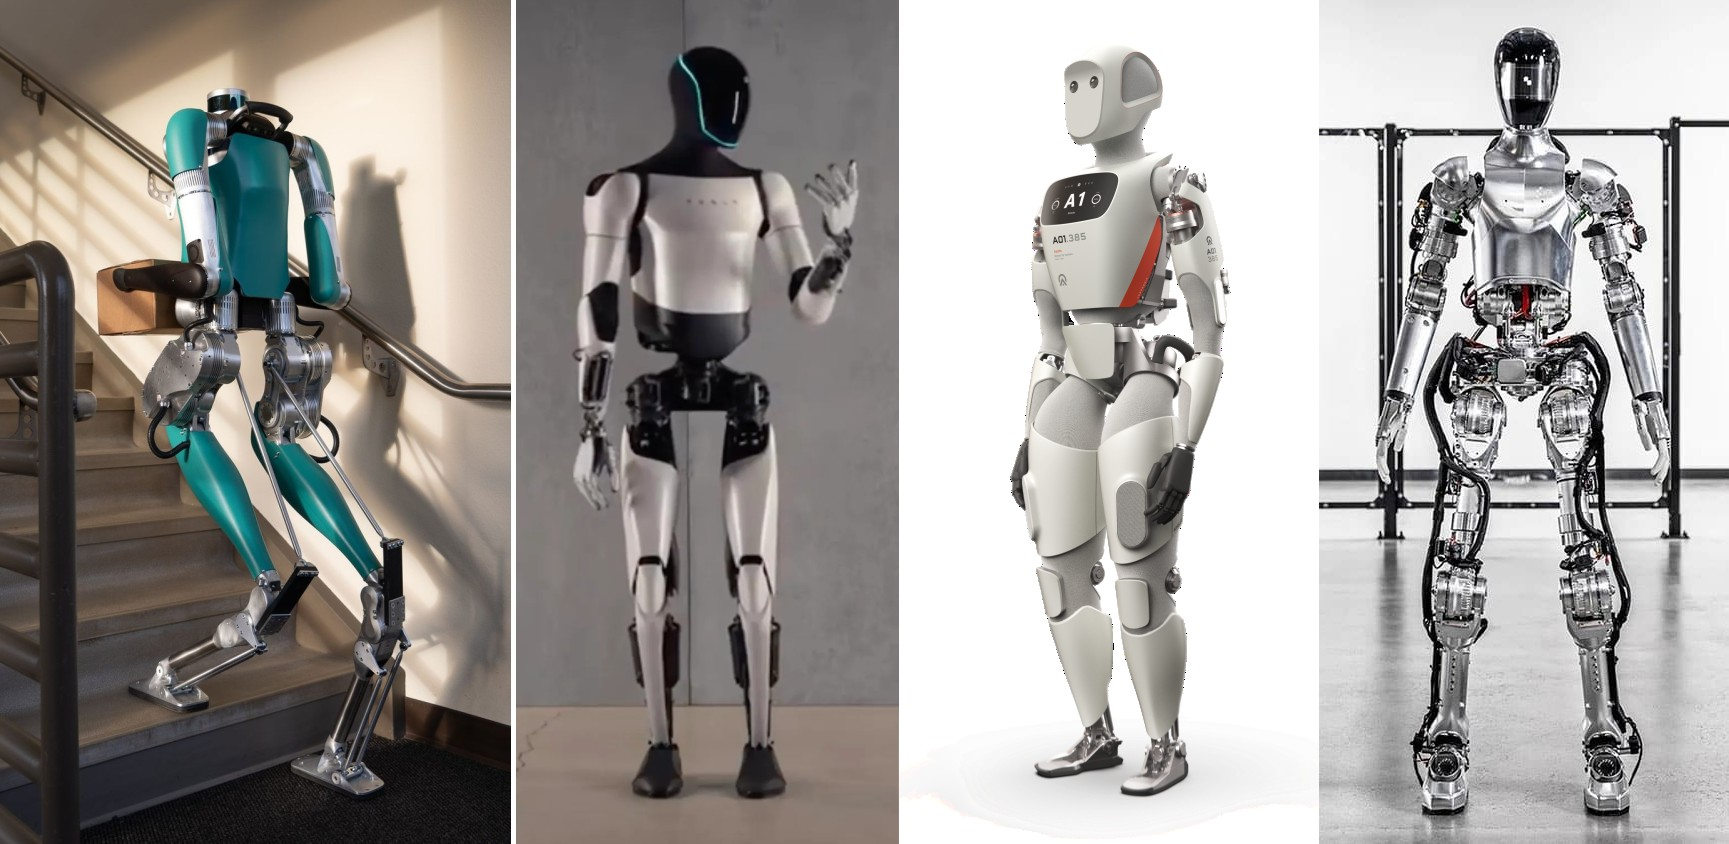
\includegraphics[width=\textwidth]{figures/01-introduction/robots-in-2020.jpg}
    \caption{Some of the humanoid robots developed in 2020s for commercial
        purposes. From left to right:
        Digit by Agility Robotics, Optimus by Tesla, Apollo by Apptronik, and
        Figure 01 by Figure AI.
    }
    \label{fig:introduction:robots-in-2020}
\end{figure}

\subsubsection{Steerable WMRs: space exploration, disaster response, human collaboration}
\begin{figure}
    \centering
    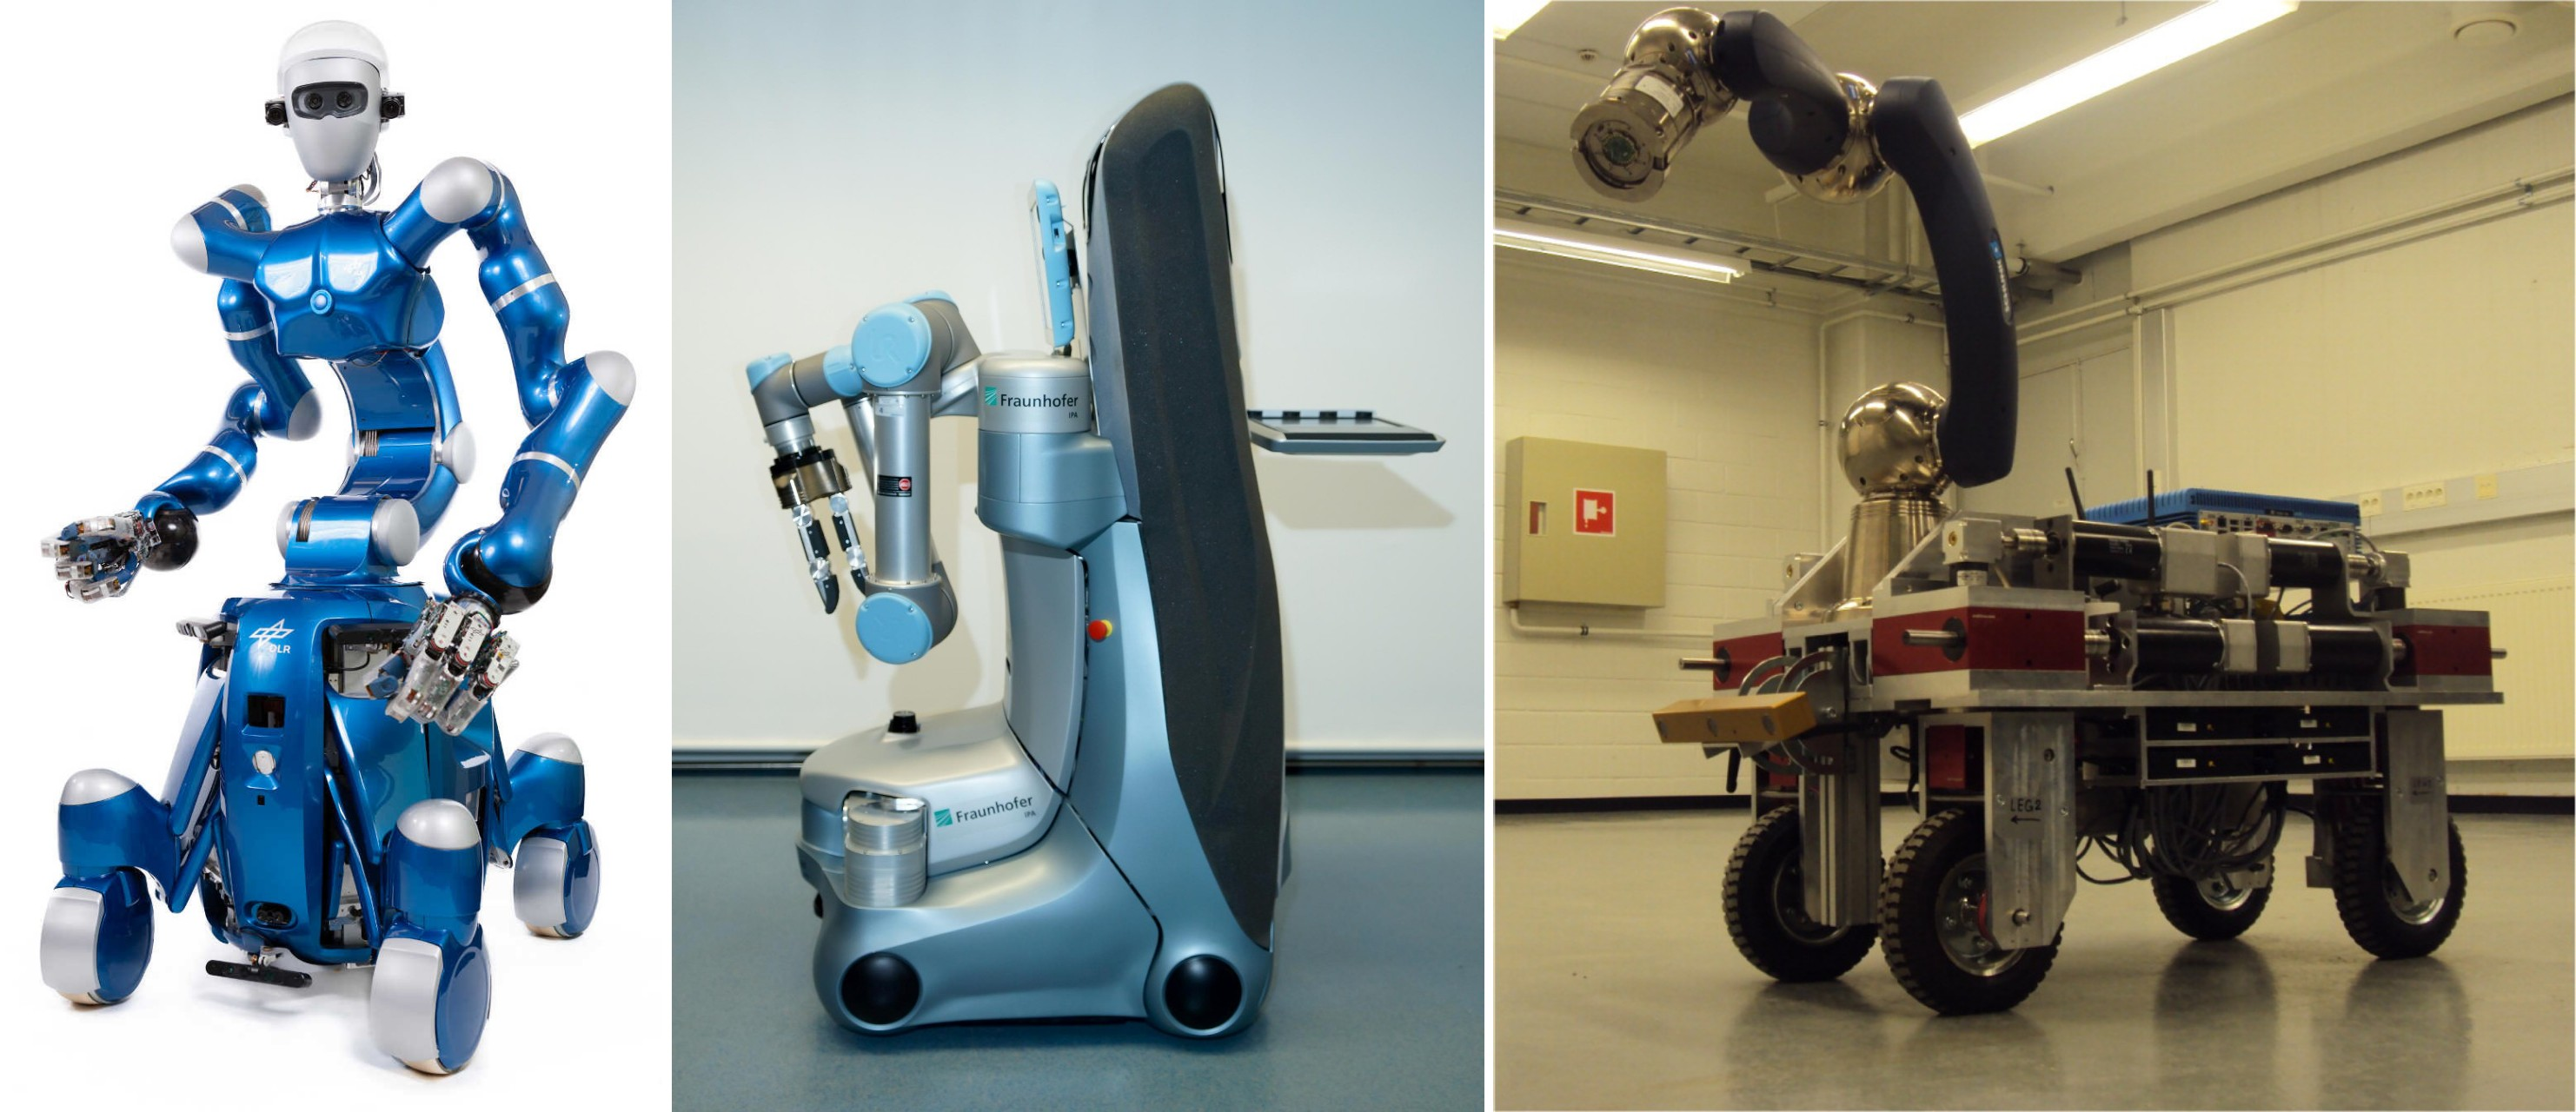
\includegraphics[width=\textwidth]{figures/01-introduction/SWMRs-1.jpg}
    \caption{Robots equipped with steerable wheels to be deployed in different areas.
        From left to right: Rollin' Justin \cite{Fuchs2009RollinJustin}, used 
        for household work and astronauts assistance in space, 
        Care-O-bot 3 \cite{Graf2009Care-O-bot3}, used as service robot, and
        iMoro \cite{Oftadeh2013iMoro}, used for inspection of contaminated
        environments.}
    \label{fig:introduction:SWMRs-1}
\end{figure}

\begin{figure}
    \centering
    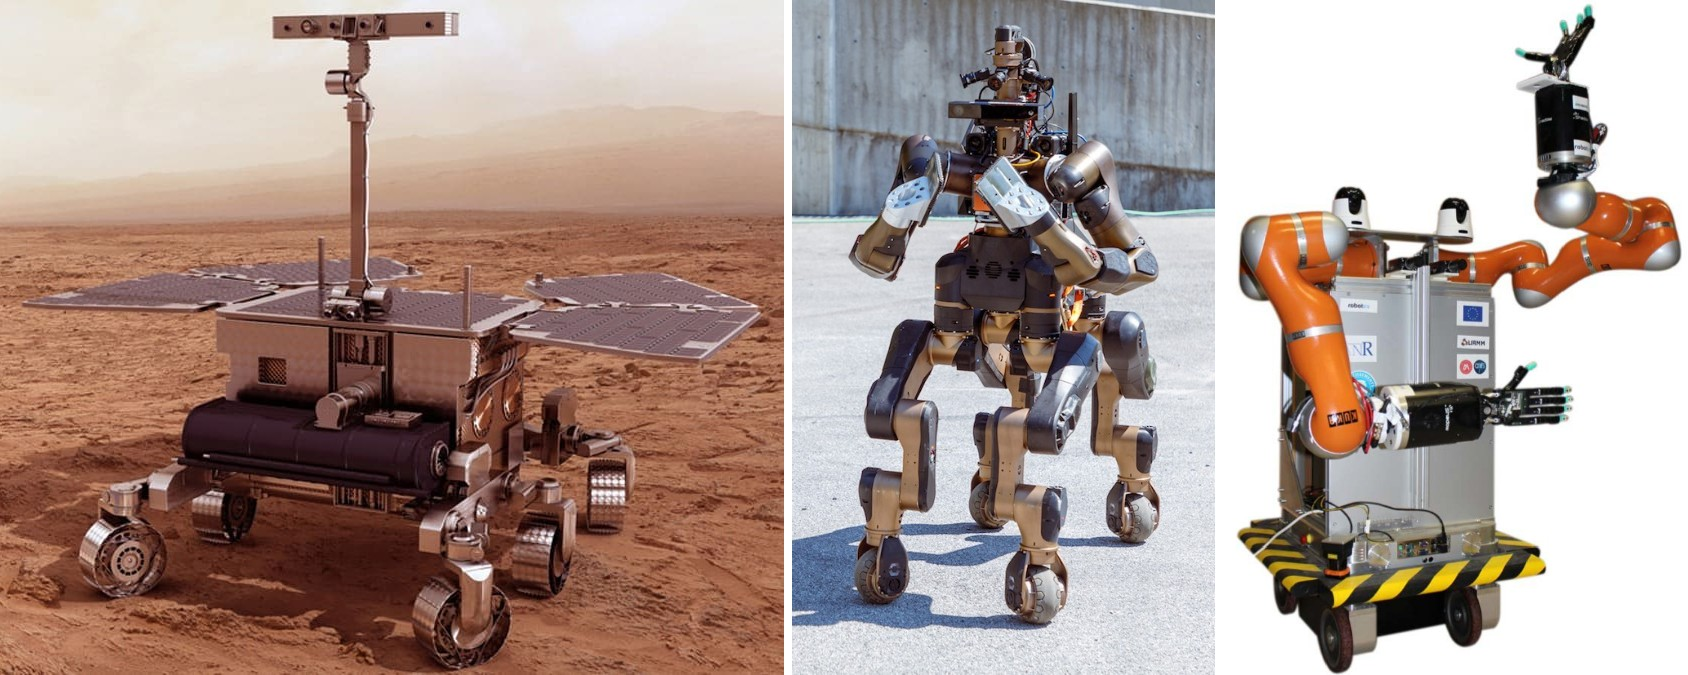
\includegraphics[width=\textwidth]{figures/01-introduction/SWMRs-2.jpg}
    \caption{More recent robots equipped with steerable wheels.
        ExoMars \cite{Poulakis2015ExoMarsMobilitySubsystem}, conceived for 
        space exploration,
        CENTAURO \cite{Kashiri2019Centauro}, designed for loco-manipulation
        in disaster scenarios, and
        BAZAR \cite{Cherubini2019ACR}, designed to interact with humans in
        assembly lines.
    }
    \label{fig:introduction:SWMRs-2}
\end{figure}
